%% abtex2-modelo-include-comandos.tex, v-1.9.5 laurocesar
%% Copyright 2012-2015 by abnTeX2 group at http://www.abntex.net.br/ 
%%
%% This work may be distributed and/or modified under the
%% conditions of the LaTeX Project Public License, either version 1.3
%% of this license or (at your option) any later version.
%% The latest version of this license is in
%%   http://www.latex-project.org/lppl.txt
%% and version 1.3 or later is part of all distributions of LaTeX
%% version 2005/12/01 or later.
%%
%% This work has the LPPL maintenance status `maintained'.
%% 
%% The Current Maintainer of this work is the abnTeX2 team, led
%% by Lauro César Araujo. Further information are available on 
%% http://www.abntex.net.br/
%%
%% This work consists of the files abntex2-modelo-include-comandos.tex
%% and abntex2-modelo-img-marca.pdf
%%

% ---
% Este capítulo, utilizado por diferentes exemplos do abnTeX2, ilustra o uso de
% comandos do abnTeX2 e de LaTeX.
% ---

\externaldocument[I-]{chapter03}

\chapter{Empirical Evaluation}\label{ch:empirical_evaluation}
\noindent
\texttt{GHS} is able to find a near-optimal and good heuristic subset to guide the A$\sp{*}$ search tree size and running time respectively, granted that it is able to compute the objective function of interest. Thus, the practical effectiveness of \texttt{GHS} depends on its ability of finding good approximations $\hat{J}$ and $\hat{T}$. In order to verify its practical effectivess, we have implemented \texttt{GHS} in Fast Downward Helmert, (\citeyear{helmert2006fast}) and tested the A$\sp{*}$ performance using subsets of heuristics selected by \texttt{GHS} while minimizing different objective funcions.

We run two sets of experiments. In the first set we verify whether the approximations $\hat{J}$ and $\hat{T}$ provided by \texttt{CS} and \texttt{SS} allow \texttt{GHS} to make near-optimal and good subset selections for A$\sp{*}$ search tree size and running time respectively. In the second set of experiments we test the effectiveness of \texttt{GHS} by measuring the total number of problem instances solved by A$\sp{*}$ using a heuristic subset selected by \texttt{GHS}.

The \texttt{GHS} is executed up to adding another heuristic does not improve the objective function. In each iteration \texttt{GHS} greedily selects from $\zeta$ the heuristic $h$ which will result in the largest reduction of the value of the objective function $\Psi$. \texttt{GHS} returns $\zeta\sp{'}$ once the objective function can not be improved.

% Please add the following required packages to your document preamble:
% \usepackage{multirow}
\begin{table}[]
\centering
\caption{Ratios of the number of nodes expanded using $h_{max}(\zeta\sp{'})$ to the number of nodes expanded using $h_{max}(\zeta)$}
\begin{tabular}{lrrrrrr}
\hline
\multirow{2}{*}{Domain} & \multicolumn{2}{c}{\texttt{SS}} & \multicolumn{2}{c}{\texttt{CS}}   & \multirow{2}{*}{|$\zeta$|} & \multirow{2}{*}{n} \\ \cline{2-5}
                        & Ratio    & |$\zeta\sp{'}$|   & Ratio  & |$\zeta\sp{'}$| &                            &                    \\ \hline
Barman                  & 1.11     & 17.70       & 1.50   & 30.25           & 5168.50                    & 20                 \\
Elevators               & 11.50     & 2.00       & 1.03   & 21.00           & 168.00                     & 1                  \\
Floortile               & 1.02     & 43.07       & 1.01   & 42.35           & 151.28                     & 14                 \\
Openstacks              & 1.00     & 1.00        & 1.00   & 1.00            & 390.69                     & 13                 \\
Parking                 & 1.00     & 5.52        & 1.01   & 7.26            & 21.73                      & 19                 \\
Pegsol                  & 1.00     & 31.00       & 1.00   & 57.00           & 90.00                      & 2                  \\
Scanalyzer              & 1.22     & 30.57       & 1.56   & 19.42           & 72.85                      & 7                  \\
Tidybot                 & 1.00     & 2.35        & 1.00   & 8.58            & 3400.17                    & 17                 \\
Transport               & 1.00     & 14.70        & 1.02   & 14.30           & 171.7                     & 10                  \\
Visitall                & 1.02     & 99.33       & 1.18   & 48.66           & 256.33                     & 3                  \\
Woodworking             & 32.42     & 3.00       & 199.65 & 5.00           & 1289.00                     & 5                  \\ \hline
\end{tabular}
\label{tb_one}
\end{table}

In all our experiments we use a type system that assigned the same type for a node with the same $f-$value. Such a type system has shown to be effective in guiding \texttt{SS} to produce accurate tree size predictions in other application domains Lelis et al., (\citeyear{lelis2013predicting}), Lelis et al., (\citeyear{lelis2014memory}).

We ran our experiments on the 2011 International Planning Competition (\texttt{IPC}) instances. We used the 2011 instances instead of the 2014 instances because the former do not have problems with conditional effects, which are currently not handled by \textbf{PDB} heuristics. All experiments are run on $2.67$ GHz machines with 4GB, and are limited to 1,800 seconds of running time.\\

% ---
\section{Empirical Evaluation of $\hat{J}$ and $\hat{T}$}
\noindent
% ---
We test whether the approximation $\hat{J}$ provided by \texttt{CS} and \texttt{SS} allows \texttt{GHS} to make near-optimal subset selections. This test is made by comparing $J(\zeta\sp{'})$ with $J(\zeta)$, which is minimal. The condition $J(\zeta\sp{'}) \leq \alpha \cdot J(\zeta)$, is sufficient to show that $J(\zeta\sp{'})$ is within $\alpha$ times good with respect to all subsets of any size, for some constant $\alpha$. We show empirically that $J(\zeta\sp{'})$ is within 10\% of $J(\zeta)$. 

In contrast with objective function $J$, there is no easy way to find the minimum of $T$ for a subset in general. We experiment then with the special case in which all heuristics in $\zeta$ have the same evaluation time. This way we are able to test whether the estimates $\hat{T}$ are allowing \texttt{GHS} to make good subset selections while minimizing the A$\sp{*}$ running time. This is because by only selecting heuristics which have the same evaluation time, if \texttt{GHS} is making near-optimal subset selections with respect to $J$, then \texttt{GHS} must also be making good subset selections with respect to $T$.

We collect values of $J(\zeta)$ and $J(\zeta\sp{'})$ as follows. For each problem instance $\nabla$ in our test set we generate a set of \texttt{PDB} heuristics using the \texttt{GA-PDB} algorithm Edelkamp, (\citeyear{edelkamp2007automated}) as described by Barley et al., (\citeyear{BarleySantiagoOver}) $-$ we call each \texttt{PDB} generated by this method a \texttt{GA-PDB}. We chose to use \texttt{GA-PDBs} in this experiment because they all have nearly the same evaluation time and will allow us to verify whether \texttt{GHS} is making near-optimal and good selections when minimizing $J$ and $T$ respectively, as explained above. The number of \texttt{GA-PDBs} generated is limited in this experiment by 1,200 seconds and 1GB of memory. Also, all \texttt{GA-PDBs} we generate have 2 millions entries each. The \texttt{GA-PDBs} generated form our $\zeta$ set. \texttt{GHS} then selects a subset $\zeta\sp{'}$ of $\zeta$. Finally, we use $h_{max}(\zeta\sp{'})$ and $h_{max}(\zeta)$ to independently try to solve $\nabla$. We call the system which uses A$\sp{*}$ with $h_{max}(\zeta)$ the \texttt{Max} approach. For \texttt{GHS} we allow 600 seconds for selecting $\zeta\sp{'}$ and for running A$\sp{*}$ with $h_{max}(\zeta\sp{'})$, and for \texttt{Max} we allow 600 seconds for running A$\sp{*}$ with $h_{max}(\zeta)$. Since we used 1,200 seconds to generate the heuristics, both \texttt{Max} and \texttt{GHS} were allowed 1,800 seconds in total for solving each problem. In this experiment we test both \texttt{CS} and \texttt{SS}.

In this experiment we refer to the approach that runs A$\sp{*}$ guided by a heuristic subset selected by \texttt{GHS} using \texttt{CS} as \texttt{GHS+CS}. Similarly, we write \texttt{GHS+SS} when \texttt{SS} is used as predictor to make the heuristic subset selection.

Table \ref{tb_one} shows the average ratios of $J(\zeta\sp{'})$ to $J(\zeta)$ for both \texttt{SS} and \texttt{CS} in different problem domains. The value of $J$, for a given problem instance, is computed as the number of nodes expanded up to the largest $f-$layer which is fully expanded by all approaches tested (\texttt{Max, GHS} using \texttt{SS} and \texttt{GHS} using \texttt{CS}). We only present results for instances that are not solved during \texttt{GHS}'s \texttt{CS} sampling process. The column $``n‘’$ shows the number of instances used to compute the averages of each row. We also show the average number of \texttt{GA-PDBs} generated (|$\zeta$|) and the average number of \texttt{GA-PDBs} selected by \texttt{GHS} (|$\zeta\sp{'}$|). This experiment shows that for most of the problems \texttt{GHS}, using \texttt{CS} or \texttt{SS}, is selecting near-optimal and a good subset of $\zeta$ for A$\sp{*}$ search tree size and running time. For example, in Tidybot \texttt{GHS} selects only a few \texttt{GA-PDBs} out of thousands when using either \texttt{SS} or \texttt{CS}. Moreover, the resulting A$\sp{*}$ search tree size is on average at most 10$\%$ larger than optimal for \texttt{GHS+SS}, and is optimal for \texttt{GHS+CS}.

The exceptions in Table \ref{tb_one} are the ratios for Elevators and Woodworking. In Woodworking \texttt{SS} has an average ratio of $32.42$ and \texttt{CS} of $199.65$. By looking at the ratios of \texttt{SS} for individual instances of \texttt{SS} for individual instances of Woodworking (results now show in Table \ref{tb_one}), we noticed that \texttt{SS} is able to make good selections for all 4 instances considered in this experiment but none of them are optimal. Since we do not know a priori what is the instance's optimal solution cost, \texttt{SS} samples nodes with $f-$values much larger than the instance's optimal solution cost. We believe that, in this particular instance of Woodworking, by sampling a portion of the state space that is not expanded during the actual A$\sp{*}$, \texttt{SS} is biasing the subset selection to select heuristics that do not contribute to reducing the actual A$\sp{*}$ search tree size.

The \texttt{SS}'s ability of sampling deep into the search space is not always harmful. For example, \texttt{SS} allows \texttt{GHS} to make good selections for instances of the Woodworking domain. By contrast, \texttt{CS}'s systematic approach to sampling only allow a shallow sample of the A$\sp{*}$ search tree. As a result, \texttt{GHS} makes a limited selection of heuristics to guide A$\sp{*}$ search. While \texttt{GHS} using \texttt{SS} selects an average of 3 heuristics in Woodworking instances, \texttt{GHS} using \texttt{CS} selects only an average of 5 heuristics. This difference on sampling strategies reflects on the number of problems solved by A$\sp{*}$. While \texttt{GHS+SS} solves 12 instances of the Woodworking domain, \texttt{GHS+CS} solves only 11. In total, out of the 280 instances of the \texttt{IPC} 2011 benchmark set, \texttt{GHS+SS} solves 199 problem instances in this experiment, while \texttt{GHS+CS} only solves 194 problem instances. (The numbers of instances solved are not shown in Table \ref{tb_one}).

\section{Comparison with Other Planning Systems}
\noindent
The objective of this second set of experiments is to test the quality of the subset of heuristics \texttt{GHS} selects while optimizing different objective functions. Our evaluation metric is coverage, \textsc{i.e.,} number of problems solved within a 1,800 second time limit. We note that the 1,800$-$second limit includes the time to generate $\zeta$, select $\zeta\sp{'}$, and run A$\sp{*}$ using $h_{max}(\zeta\sp{'})$. The $\zeta$ set of heuristics is composed of a number of different \texttt{GA-PDBs}, a \texttt{PDB} heuristic produced by the \texttt{iPDB} method Haslum et al., (\citeyear{haslum2007domain}) and the \texttt{LM-Cut} heuristic. The generation of \texttt{GA-PDBs} is limited by 600 seconds and 1GB of memory. We use one fourth of 600 seconds to genetate \texttt{GA-PDBs} with each of the following number of entries: $\{2 \cdot 10\sp{3}, 2 \cdot 10\sp{4}, 2 \cdot 10\sp{5}, 2 \cdot 10\sp{6}\}$. Our approach allows one to generate up to thousands of \texttt{GA-PDBs}. For every problem instance, we use exactly the same $\zeta$ set for \texttt{Max} and all \texttt{GHS} approaches.

\section{Systems Tested}
\noindent
\texttt{GHS} is tested while minimizing the A$\sp{*}$ search tree size (\texttt{Size}) and the A$\sp{*}$ running time (\texttt{Time}). We also use \texttt{GHS} to maximize the sum of heuristic values in the state space (\texttt{Sum}), as suggested by Rayner et al., (\citeyear{raynersss13}). Rayner et al., (\citeyear{raynersss13}) assumed that one could uniformly sample states in the state space in order to estimte the sum of the heuristic values for a given heuristic subset. Since we are not aware of any method to uniformly sample the state space of domain$-$independent problems, we adapted the Rayner et al., (\citeyear{raynersss13})'s method by using \texttt{SS} to estimate the sum of heuristic values in the search tree rooted at $\nabla$'s start state. We write \texttt{Size + SS} to refer to the approach that used A$\sp{*}$ guided by a heuristic selected by \texttt{GHS} while minimizing an estimate of the search tree size provided by \texttt{SS}. We follow the same pattern to name the other possible combinations of objective functions and prediction algorithms (\textsc{e.g.,}\texttt{Time+CS}).

In addition to experimenting with all combination of prediction algorithms (\texttt{CS} and \texttt{SS}) and objective functions (\texttt{Time}, \texttt{Size}), we also experiment with an approach that minimizes both the search tree size and the running time as follows. First we create a pool of heuristics $\zeta$ composed solely of \texttt{GA-PDB} heuristics, then we apply \texttt{GHS} while minimizing tree size and using \texttt{SS} as predictor. As explained above, in this setting \texttt{GHS} minimizes $J$ and $T$ simultaneaously, as all heuristics in $\zeta$ have the same evaluation time. We call the selection of a subset of \texttt{GA-PDBs} as the \textit{first selection}. Once the first selection is made, we test all possible combinations of the resulting $h_{max}(\zeta\sp{'})$ added to the \texttt{iPDB} and \texttt{LM-Cut} heuristics while minimizing the running time as estimated by \texttt{CS}$-$we call this step the \textit{second selection}. We call the overall approach \texttt{Hybrid}.

The intuition behind \texttt{Hibrid} is that we apply \texttt{GHS} with its strongest settings. \texttt{GHS} makes near-optimal and good selections respect to $J$ and $T$ respectively when selecting from a pool of heuristics with the same evaluation time. After such a selection is made, we reduce the size of the pool of heuristics from possible thousands to only three (the maximum of a subset of the initial \texttt{GA-PDBs, iPDB}, and \texttt{LM-Cut}). With only three heuristics we are able to choose the exact combination that minimizes the A$\sp{*}$ running time the most. The reason we chose to use \texttt{SS} instead of \texttt{CS} for the first selection in \texttt{Hybrid} is that the former is able to make better subset selections in this setting, as suggested by the results discussed in the previous Chapter \ref{ch:rghs}. Finally, as we show below, \texttt{CS} is more effective if one is interested in minimizing the A$\sp{*}$ running time while selecting from a pool of heuristic with different evaluation times. That is why we use \texttt{CS} as predictor for the second selection in \texttt{Hybrid}.

We compare the coverage of the \texttt{GHS} approaches with several other state$-$of$-$the$-$art planners. Namely, we experiment with RIDA$\sp{*}$ Barley et al., (\citeyear{BarleySantiagoOver}), two variants of StoneSoup (StSp1 and StSp2) as described by Nissim et al., (\citeyear{nissim2011computing}), two versions of Symba (SY1 and SY2), and A$\sp{*}$ being independently guided by the maximum of all heuristics in $\zeta$ (\texttt{Max}), \texttt{iPDB, LM-cut} and \texttt{Merge $\&$ Shrink}(\texttt{M$\&$S}) Nissim et al., (\citeyear{nissim2011computing}).

The results are presented in Table \ref{tb_two}. The results for the \texttt{GHS} approaches are averages computed over 10 independent runs of the planner; the average numbers are truncated to two decimal places in our table. The variance of the results is small, thus we omitted them from the table of results.

\section{Discussion of the Results}
\noindent
The system that solves the largest number of instances is \texttt{Hybrid}$-$ it solves 219 problems on average. As explained above, we combine in \texttt{Hybrid} the strengths of both \texttt{SS} and \texttt{CS} in a single system. \texttt{SS} is used to greedily select heuristics from a pool of heuristics with similar evaluation time, and only then \texttt{CS} is used for selecting heuristics with different evaluation times. This strategy has proven particularly effective on the Barman domain where \texttt{Hybrid}'s first selection is able to select near-optimal subsets of \texttt{GA-PDBs} and its second selection is able to recognize that it must not include the \texttt{iPDB} and \texttt{LM-Cut} heuristics to the subset selected by its first selection. As a result, \texttt{Hybrid} solves more problems on this domain than any other \texttt{GHS} approach.

\texttt{Time+CS} also performed well in our experiments$-$the approach solves 216 problems on average. Clearly \texttt{Hybrid} and \texttt{Time+CS} are far superior to all other approaches tested. For example, \texttt{Size + SS} and \texttt{Sum} solves only 206 and 207 problems, respectively. While minimizing the search tree size or maximizing the sum of heuristic values, \texttt{GHS} will tend to add accurate heuristics to the selected subset, independently of their evaluation time. As a result, if not minimizing the running time, \texttt{GHS} often adds the \texttt{LM-Cut} heuristic to $\zeta\sp{'}$ as \texttt{LM-Cut} is often the heuristic that is able to reduce the most the search tree size and to increase the most the sum of heuristic values. However, \texttt{LM-Cut} is very computationally expensive, and in various cases the search is faster if \texttt{LM-Cut} is not in $\zeta\sp{'}$. Both \texttt{Hybrid} and \texttt{Time+CS} are able to recognize when \texttt{LM-Cut} should not be included in $\zeta\sp{'}$ because they account for the heuristics' evaluation time.

% Please add the following required packages to your document preamble:
% \usepackage{multirow}
\begin{table}[htb]
\footnotesize\setlength{\tabcolsep}{1.8pt}
\centering
\caption{Coverage of different planning systems on the 2011 \texttt{IPC} benchmarks. For the \texttt{GHS} and \texttt{Max} approaches we also present the average number of heuristics \texttt{GHS} selects (|$\zeta\sp{'}$|).}
\begin{tabular}{lrrrrrrrrrrrrrrr}
\hline
\multirow{2}{*}{Domains} & \multirow{2}{*}{\texttt{Hybrid}} & \multicolumn{2}{c}{\texttt{CS}} & \multicolumn{2}{c}{\texttt{SS}} & \multirow{2}{*}{\texttt{Sum}} & \multirow{2}{*}{RIDA$\sp{*}$} & \multirow{2}{*}{SY1} & \multirow{2}{*}{SY2} & \multirow{2}{*}{StSp1} & \multirow{2}{*}{StSp2} & \multirow{2}{*}{\texttt{Max}} & \multirow{2}{*}{iPDB} & \multirow{2}{*}{LM-Cut} & \multirow{2}{*}{M$\&$S} \\ \cline{3-6}
                         &                                    & \texttt{Time} & \texttt{Size} & \texttt{Time} & \texttt{Size} &                                 &                       &                      &                      &                        &                        &                                 &                       &                         &                         \\ \hline
Barman&         7&     16&     4&    4&    4&   4&   4&   10&   11&   4&   4&    4&   4&   4&   4\\
Elevators&     19&     14&    19&   19&   19&  19&  19&   20&   20&  18&  18&   19&  17&  18&  12\\
Floortile&     14&     15&    14&   14&   14&  14&  14&   14&   14&  14&  14&   14&   8&  14&  10\\
Nomystery&     20&     19&    20&   19&   20&  20&  20&   16&   16&  20&  20&   20&  19&  14&  18\\
Openstacks&    17&     19&    15&   17&   15&  15&  15&   20&   20&  17&  17&   11&  17&  15&  17\\
Parcprinter&   18&     14&    15&   16&   16&  19&  18&   17&   17&  18&  18&   18&  16&  17&  16\\
Parking&        7&     20&     2&    7&    2&   2&   7&    2&    1&   5&   5&    2&   7&   2&   7\\
Pegsol&        19&     20&    19&   19&   19&  19&  19&   19&   20&  19&  19&   19&  20&  17&  19\\
Scanalyzer&    14&     18&    13&   11&   14&  14&  14&    9&    9&  14&  14&   14&  10&  12&  11\\
Sokoban&       20&     19&    20&   20&   20&  20&  20&   20&   20&  20&  20&   20&  20&  20&  20\\
Tidybot&       16&      4&    16&   16&   17&  16&  17&   15&   17&  16&  16&   15&  14&  16&   9\\
Transport&     14&     14&    13&   11&   13&  11&  10&   10&   11&   7&   8&    9&   8&   6&   7\\
Visitall&      18&      7&    17&   15&   17&  18&  18&   12&   12&  16&  16&   18&  16&  10&  16\\
Woodworking&   16&     17&    16&   12&   16&  16&  15&   20&   20&  15&  15&   16&   9&  15&   9\\ \hline
Total&        219&    216&   203&  200&  206& 207& 210&  204&  208& 203& 204&  199& 185& 180& 175\\ \hline
\end{tabular}
\label{tb_two}
\end{table}

Note that the difference on the number of problems solved by \texttt{Time+CS} and \texttt{Time+SS}: While the former solves 216 instances, the latter solved only 200. We conjecture that this happens because \texttt{SS} is not able to detect duplicated nodes during sampling. As a result, \texttt{SS} often overestimates by several orders of magnitude the actual A$\sp{*}$'s running time. Similarly to the \texttt{Size} and \texttt{Sum} approaches, due to \texttt{SS}'s overestimations, \texttt{Time+SS} often mistakenly adds the accurate but expensive \texttt{LM-Cut} heuristic in cases where the A$\sp{*}$ search would be faster without \texttt{LM-Cut}'s guidence. For example, although \texttt{iPDB} tends to prune fewer nodes than \texttt{LM-Cut} in Parking instances, \texttt{iPDB} is the heuristic of choice in that domain. This is because its evaluation time is much smaller than \texttt{LM-Cut}'s. \texttt{Time+CS} solves 20 Parking instances on average as it correctly selects \texttt{iPDB} and leaves \texttt{LM-Cut} out of $\zeta\sp{'}$. By contrast, likely due to its prediction overestimation, \texttt{Time+SS} solves 7 parking instances because wrongly estimates \texttt{LM-Cut} that will reduce overall search time and adds the heuristic to its selected subset. Notice, that \texttt{Size+CS} and \texttt{Size+SS} also does poorly Parking instances as they also always select \texttt{LM-Cut}.

RIDA$\sp{*}$ is the most similar system to \texttt{GHS}, as it also selects a subset of heuristics from a pool of heuristics by using an evaluation method similar to \texttt{CS}. RIDA$\sp{*}$ uses a systematic approach for selecting a subset of heuristics. Namely, it starts with an empty subset and evaluates all subsets of size $i$ before evaluating subsets of size $i+1$. This procedure allows RIDA$\sp{*}$ to consider only tens of heuristics in their pool. By contrast, \texttt{GHS} is able to consider thousands of heuristics while making its selection.

The ability to handle large set of heuristics can be helpful, even if most of the heuristics in the set are redundant with each other$-$as is the case with the \texttt{GA-PDBs}. The process of generating \texttt{GA-PDBs} is stochastic, thus one increases the chances of generating helpful heuristic by generating a large number of them. \texttt{GHS} is an effective method for selecting a small set of informative heuristics from a large set of mostly uninformative ones. This is illustrated in Table \ref{tb_two} on the Transport domain. Compared to systems which use multiple heuristics (StSp1 and 2, and RIDA$\sp{*}$), \texttt{Time+CS} solves the largest number of Transport instances, which is due to the selection of a few key \texttt{GA-PDBs}.

The best \texttt{GHS} approach, \texttt{Hybrid}, substantially outperforms the number of instances solved by \texttt{Max$-$Hybrid} solves on average more than 20 instances than \texttt{Max}. Finally, \texttt{Hybrid} and \texttt{Time+CS} substantially outperforms all other approaches tested, with RIDA$\sp{*}$ being the closest competitor with 210 instances solved.

\section{Comparison between SS and IDA*}
\noindent
In this experiment \texttt{SS} estimates the search tree size generated by IDA$\sp{*}$ using a consistent heuristic. \texttt{SS} estimates the size of the search tree up to some defined deep $f$-layer in the tree.

We first ran IDA$\sp{*}$ for Fast-Downward benchmark for optimal domains. Our evaluation metric is coverage, \texttt{i.e.,} number of problems solved within 30 minutes time limit. We note that in 30 minutes non all the instances for a specific domain using a consistent heuristic can be solved. Afterwards, run \texttt{SS} using as a threshold the $f-$layer limited by the search time, this process is executed using different number of probes \texttt{i.e.,} 1, 10, 100, 1000 and 5000.

\begin{equation}
\frac{\sum_{s\in PI} \frac{Pred(s, d) - R(s, d)}{R(s, d)}}{|PI|}
\label{eq:eq_comparison}
\end{equation}

The Formula \ref{eq:eq_comparison} is called relative-error, this help us to determinate the accuracy of the prediction of \texttt{SS} about IDA$\sp{*}$ given a state $s$ and cost bound $d$. The parameters that this Formula require are:

\begin{itemize}
  \item $PI$ is the set of instances.
  \item $Pred(s,d)$ is the predicted number of nodes expanded by IDA$\sp{*}$ for start state $s$ and cost bound $d$.
  \item $R(s,d)$ is the actual number of nodes expanded by IDA$\sp{*}$ for start state $s$ and cost bound $d$.
\end{itemize}

The result from apply the relative-error is a number, that in order to obtain a good approximation, the result must be near to $0.00$, which represent the perfect score.

The Table \ref{tb:comparison} shows how the relative-error behavies when \texttt{SS} makes prediction of the number of nodes expanded by IDA$\sp{*}$ when it is searching with a specific heuristic and cost threshold. The heuristic used in this experiment is $hmax$. Five probes were used: 1, 10, 100, 1000 and 5000. The average value of IDA$\sp{*}$ and time were used. The relative-error gets a perfect score while increasing the number of probes. For Barman, the relative-error goes from $0.60$ for 1 probe to $0.45$ for 10 probes, $0.20$ for 100 probes, $0.07$ for 1000 probes and $0.04$ for 5000 probes. In the case of time, while the number of probes increase, \texttt{SS} need to spend more time calculating the size of the search tree. Then, the time increase. For Barman, the time goes from $0.06\ seconds$ for 1 probe to $0.32\ seconds$ for 10 probes, $3.21\ seconds$ for 100 probes, $32.57\ seconds$ for 1000 probes and $214.59\ seconds$ for 5000 probes. There are domains such as: Parcprinter, Parking, Pegsol and Visitall that have perfect score using 5000 probes. In the case of Tidybot, the relative-error using 1 probe is smaller than using 10 probes. The reason might be the search tree generated for some instances or the stochastic behavior of \texttt{SS} that sometimes it will choose a node that expand a search tree that will be more expensive to expand. The last column \textsf{n} represent the number of instances where IDA$\sp{*}$ found the number of nodes expanded when it is searching with $hmax$ and cost threshold. The 2011 \texttt{IPC} domains contains 20 instances per domain. Floortile only have 2 instances, it means that when running IDA$\sp{*}$ for all the instances of Floortile only two instances (opt-p01-001.pddl and opt-p03-006.pddl) have found number of nodes expanded under some threshold. In summary, we proved that for 2011 \texttt{IPC} domains, \texttt{SS} estimations converges to the real search tree size generated by IDA$\sp{*}$ when the number of probes goes to infinity.

% Please add the following required packages to your document preamble:
% \usepackage{multirow}
\begin{table}[]
%\footnotesize\setlength{\tabcolsep}{1.2pt}
\tiny\setlength{\tabcolsep}{2pt}
\centering
\caption{Comparison between \texttt{SS} and IDA$\sp{*}$ for 1, 10, 100, 1000 and 5000 probes using $hmax$ heuristic.}
\label{tb:comparison}
\begin{tabular}{lrrrrrrrrrrrrr}
\hline
\multirow{3}{*}{Domain} & \multicolumn{13}{c}{$hmax$}                                                                                                                     \\ \cline{2-14} 
                        & \multirow{2}{*}{IDA$\sp{*}$} & \multirow{2}{*}{time} & \multicolumn{5}{c}{relative$-$error} & \multicolumn{5}{c}{time}   & \multirow{2}{*}{n} \\ \cline{4-13}
                        &                              &                       & 1   & 10   & 100   & 1000   & 5000   & 1 & 10 & 100 & 1000 & 5000 &                    \\ \hline
Barman & 8835990.00& 6016.38& 0.60& 0.45& 0.20& 0.07& 0.04& 0.06& 0.32& 3.21& 32.57& 214.59& 20\\
Elevators & 1012570.00& 4987.57& 0.84& 0.42& 0.23& 0.13& 0.10& 1.40& 9.85& 96.37& 994.33& 4425.93& 20\\
Floortile & 30522300.00& 3919.72& 2.02& 0.62& 0.40& 0.14& 0.11& 0.01& 0.07& 0.69& 6.93& 36.60& 2\\
Nomystery & 6565740.00& 3256.86& 0.53& 0.26& 0.07& 0.03& 0.01& 0.07& 0.38& 3.63& 36.35& 181.03& 20\\
Openstacks & 80108.50& 4017.19& 0.03& 0.03& 0.03& 0.03& 0.03& 94.79& 774.86& 1067.84& 10929.00& 11174.30& 20\\
Parcprinter & 1.00& 0.00& 0.00& 0.00& 0.00& 0.00& 0.00& 0.01& 0.04& 0.35& 3.48& 17.29& 20\\
Parking & 374925.00& 5607.50& 0.17& 0.04& 0.01& 0.00& 0.00& 1.79& 11.36& 114.28& 1196.83& 5835.03& 20\\
Pegsol & 68763.70& 5.00& 0.17& 0.04& 0.02& 0.01& 0.00& 0.01& 0.04& 0.37& 3.69& 17.88& 20\\
Scanalyzer & 8449890.00& 4920.58& 0.43& 0.25& 18.63& 0.02& 0.01& 3.13& 28.79& 273.74& 3033.06& 10254.00& 20\\
Sokoban & 3118530.00& 3932.69& 0.41& 0.26& 0.11& 0.05& 0.04& 0.31& 2.00& 21.42& 222.47& 1056.61& 20\\
Tidybot & 444473.00& 5632.08& 300.86& 1072.40& 5.88& 0.01& 0.01& 4.40& 26.48& 238.76& 2747.10& 11925.40& 20\\
Transport & 2622880.00& 2253.51& 0.63& 0.54& 0.24& 0.15& 0.11& 0.09& 0.61& 5.89& 59.37& 290.31& 20\\
Visitall & 71032400.00& 3704.78& 0.12& 0.04& 0.01& 0.00& 0.00& 0.00& 0.05& 0.56& 5.77& 28.07& 20\\
Woodworking & 5139070.00& 4944.76& 1.28& 0.69& 0.27& 0.17& 0.07& 0.15& 1.33& 13.21& 130.82& 664.08& 20\\ \hline
\end{tabular}
\end{table}

\section{Comparison between SS and A*}
\noindent
The Table \ref{tb:ipdb_lmcut_mands} shows that \texttt{SS} is not a good estimator for A$\sp{*}$ and that is because \texttt{SS} does not count for duplicate nodes and A$\sp{*}$ does. \texttt{SS} overestimate the A$\sp{*}$ search tree size. As a result, \texttt{SS} often gets values by several orders of magnitude bigger than the actual A$\sp{*}$ search tree.

% Please add the following required packages to your document preamble:
% \usepackage{multirow}
\begin{table}[!htb]
\footnotesize\setlength{\tabcolsep}{1.2pt}
\centering
\caption{Poor prediction of SS against A* using ipdb, \texttt{LM-Cut} and M$\&$S with 500 probes}
\label{tb:ipdb_lmcut_mands}
\begin{tabular}{lR{2cm}R{2cm}R{2cm}R{2cm}R{2cm}R{2cm}C{2cm}}
\hline
\multirow{2}{*}{Domain} & \multicolumn{2}{c}{ipdb} & \multicolumn{2}{c}{\texttt{LM-Cut}} & \multicolumn{2}{c}{M$\&$S} & \multirow{2}{*}{n} \\ \cline{2-7}
                     & A*          & SS$-$error         & A*                & SS$-$error                & A*           & SS$-$error          &                    \\ \hline
Barman               & 1.72e+07    & 8.68e+31   & 7.45e+06          & 2.21e+30          & 6.67e+06     & 1.26e+36    & 4                  \\
Floortile            & 1.40e+07    & 1.74e+18   & 702435            & 4.68e+14          & 4.46e+06     & 1.90e+12    & 4                  \\
Nomystery            & 40169.7     & 6.71e+32   & 267100            & 6.14e+19          & 8236         & 1.20e+20    & 9                  \\
Openstacks           & 570099      & 0.61884    & 570099            & 0.677425          & 569984       & 0.672143    & 4                  \\
Parcprinter          & 1157        & 2.56e+22   & 1363.67           & 2.33e+21          & 766.333      & 6.36e+20    & 3                  \\
Pegsol               & 841693      & 2901.39    & 398221            & 6859.86           & 933430       & 779.017     & 16                 \\
Scanalyzer           & 337894      & 3.94e+33   & 334747            & 7.58e+31          & 337833       & 2.42e+31    & 3                  \\
Sokoban              & 376755      & 1.04e+07   & 45374             & 2.74e+06          & 739775       & 5.60e+08    & 9                  \\
Transport            & 1.89e+06    & 2.91e+38   & 1.49e+06          & 1.15e+25          & 1.73e+06     & 1.50e+29    & 2                  \\
Visitall             & 253710      & 1.69e+46   & 253195            & 1.69e+46          & 253521       & 1.71e+46    & 8                  \\
Woodworking          & 3.21e+06    & 2.53e+18   & 3.20e+06          & 2.76e+18          & 3.21e+06     & 2.48e+18    & 3                  \\ \hline
\end{tabular}
\end{table}

Three heuristics were used: ipdb, \texttt{LM-Cut} and M$\&$S.  The last column \textsf{n} represent the number of instances solved by A$\sp{*}$ using the three heuristics. For this experiment we decided to use only the instances that are solved by the three heuristics at the same time. The columns with A$\sp{*}$ represents the average of number of nodes expanded by A$\sp{*}$ using a specific heuristic. The column with \texttt{SS}-error represents the relative-error Formula \ref{eq:eq_comparison}.

For Barman: Using M$\&$S, A$\sp{*}$ expands in average 6.67e$+$06 which is less nodes than ipdb$-$1.72e$+$07 and \texttt{LM-Cut}$-$7.45e$+$06. However, using M$\&$S, \texttt{SS}$-$error is 1.26e$+$36, ipdb$-$8.68e$+$31 and \texttt{LM-Cut}$-$2.21e$+$30. Which indicates that the number of nodes expanded by \texttt{SS} in average is in the order of magnitude of 30 to 40. In Visitall, \texttt{SS}-error shows that \texttt{SS} overestimates A$\sp{*}$ highly, which represent a very bad prediction of \texttt{SS}. In Openstack: Using the three heuristics, A$\sp{*}$ expands almost the same number of nodes for the 4 instances solved. And \texttt{SS}-error shows a score near to the perfect and the reason is because \texttt{SS} expands less nodes than A$\sp{*}$.

\section{Approximation Analysis for SS and A*}
\noindent
Here we show that \texttt{SS} is able to make near-optimal selection of heuristics ipdb, \texttt{LM-Cut} and \texttt{GA-PDBs} with respect to the A$\sp{*}$ search tree size.

Moreover, in order to understand how \texttt{SS} and A$\sp{*}$ behaves we have created plots with the fixed range of 2. This way we are going to have 4 different regions as shown in the Figure \ref{fig:img_cartesian_plane} . The points represent the fraction between the  number of nodes expanded by A$\sp{*}$ using a heuristic $i$ ($J(h_{i})$), and the estimate of the number of nodes expanded by \texttt{SS} ($\hat{J}(h_{i})$). Points on regions II and III are heuristics that \texttt{SS} correctly choose to be used with A$\sp{*}$. Points following on the other regions are those choices, \texttt{SS} made incorrectly.

Points that fall in each of the regions:
\begin{enumerate}[label=\Roman*]
\item $J(h_{2}) > J(h_{1})$ for A$\sp{*}$, $\hat{J}(h_{1}) > \hat{J}(h_{2})$ according to \texttt{SS}. 
\item $J(h_{2}) > J(h_{1})$ for A$\sp{*}$ and \texttt{SS} agrees.
\item $J(h_{1}) > J(h_{2})$ for A$\sp{*}$ and \texttt{SS} agrees.
\item $J(h_{1}) > J(h_{2})$ for A$\sp{*}$, $\hat{J}(h_{2}) > \hat{J}(h_{1})$ according to \texttt{SS}.
\end{enumerate}

\pagestyle{empty}

\begin{figure}[!htb]
\centering  
\begin{tikzpicture}[scale=2]
  \draw[->] (-0.2,0) -- (3,0) node[right] {\texttt{SS} $-$ ($\hat{J}(h_{1})$/$\hat{J}(h_{2})$)};
  \draw[->] (0,-0.2) -- (0,3) node[above] {A$\sp{*}$ $-$ ($J(h_{1})$/$J(h_{2})$)};

  \draw[densely dotted] (-0.1,1) -- (3,1);
  \draw[densely dotted] (1,-0.1) -- (1,3);
  
  \draw[densely dotted] (-0.1,2) -- (3,2);
  \draw[densely dotted] (2,-0.1) -- (2,3);

  \draw[shift={(0.5,1.5)}] node[below] {I};
  \draw[shift={(1.5,1.5)}] node[below] {II};
  \draw[shift={(0.5,0.5)}] node[below] {III};
  \draw[shift={(1.5,0.5)}] node[below] {IV};


  \foreach \x/\xtext in {1/1, 2/2}
    \draw[shift={(\x,0)}] (0pt,2pt) -- (0pt,-2pt) node[below] {$\xtext$};

  \foreach \y/\ytext in {1/1, 2/2}
    \draw[shift={(0,\y)}] (2pt,0pt) -- (-2pt,0pt) node[left] {$\ytext$};

\end{tikzpicture}
  \caption{Cartesian Plane with domain $\left\langle 0, 2\right\rangle$ and range $\left\langle 0, 2\right\rangle$ }\label{fig:img_cartesian_plane}
\end{figure}

In the Figure \ref{fig:img_analysis_domains} we can see the distribution of the points in each domain. We use three different heuristics ratios: ipdb, \texttt{LM-Cut}(lmcut) and 10 \texttt{GA-PDBs}(gapdb) which are represented by the symbols \ding{110} , \ding{108} and \ding{115} respectively. The ipdb ratio is the result of divide two search tree size generated by $h_{1} =$ ipdb and $h_{2} =$ ipdb. The \texttt{LM-Cut} ratio is the result of divide two search tree size generated by $h_{1} =$ \texttt{LM-Cut} and $h_{2} =$  \texttt{LM-Cut}. When at least one heuristic $h_{1}$ or $h_{2}$ is \texttt{GA-PDB} then the heuristic ratio is \texttt{GA-PDB}. This experiment was done using 5000 probes for \texttt{SS} and during 30 minutes.

The eleven plots displayed show the distribution of the heuristic ratios in the four quadrants. We drew the function $y = x$ because \texttt{SS} yields a perfect fraction if the point fall in that function. That is why it is important to have such a line as a reference on the plot. We decided to use the same scale on both axis. Otherwise it will be hard to see which points fall on the diagonal line ($y = x$) and which points don't. Furthermore, the scale is $2$ for both axis. So, the points that are far away from the quadrants, are set to be in the limit. For example, if any of the ratios $r$ is larger than $1,000$ then $r$ will be on the $2$ border of the plot.

The points $(0,0), (1,1), (2,2)$ mean that \texttt{SS} made a perfect choice and these points represent the function $y = x$. As we are interested in the percentage of points that fall in the quadrants II and III we are going to consider the border only for those quadrants.

The points are dispersed in the positive quadrant of the cartesian plane because we do not have negative number of nodes generated by $h_{1}$ or $h_{2}$. In the case of Tidybot and Woodworking all the points are in the quadrant II or III.

\begin{figure}[!htb]
\minipage{0.32\textwidth}
  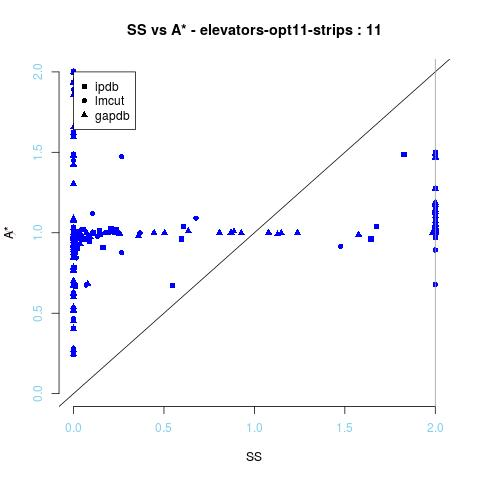
\includegraphics[width=\linewidth]{images/elevators-opt11-strips}
\endminipage\hfill
\minipage{0.32\textwidth}
  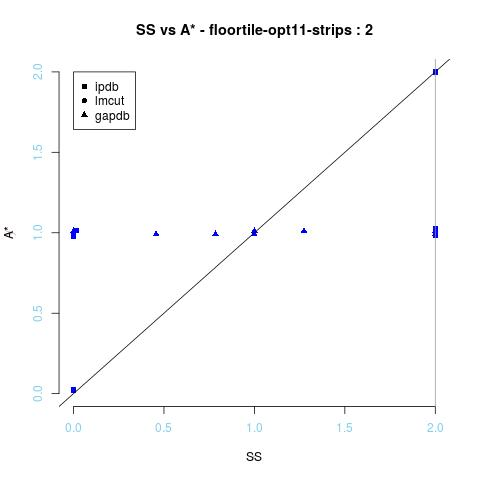
\includegraphics[width=\linewidth]{images/floortile-opt11-strips}
\endminipage\hfill
\minipage{0.32\textwidth}%
  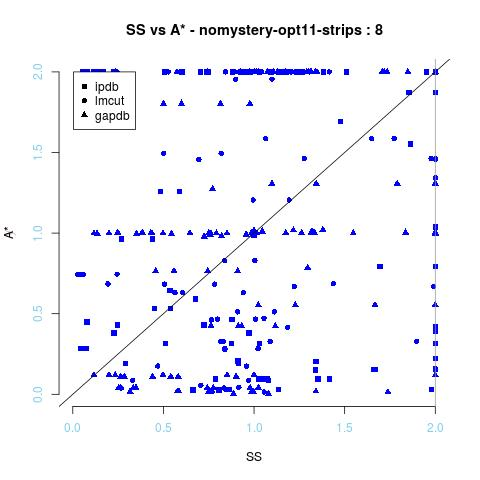
\includegraphics[width=\linewidth]{images/nomystery-opt11-strips}
\endminipage

%jump
\minipage{0.32\textwidth}
  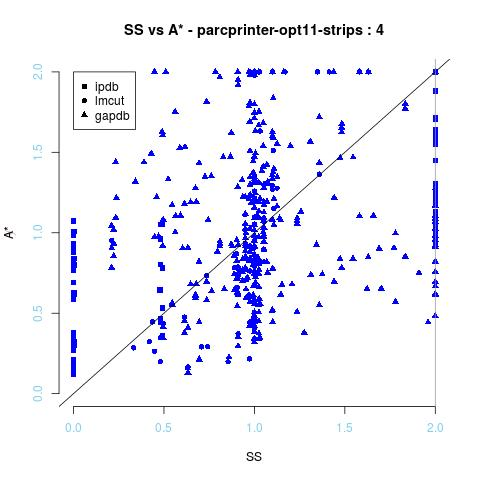
\includegraphics[width=\linewidth]{images/parcprinter-opt11-strips}
\endminipage\hfill
\minipage{0.32\textwidth}
  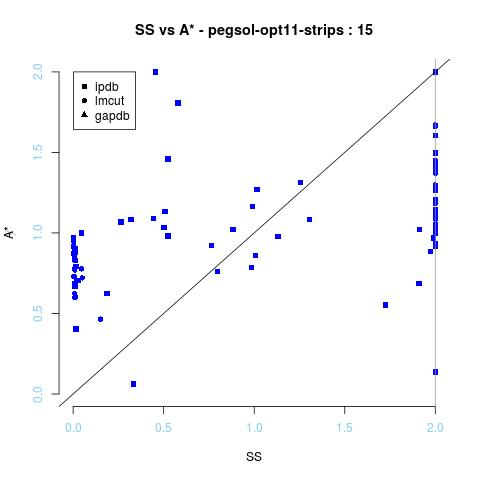
\includegraphics[width=\linewidth]{images/pegsol-opt11-strips}
\endminipage\hfill
\minipage{0.32\textwidth}
  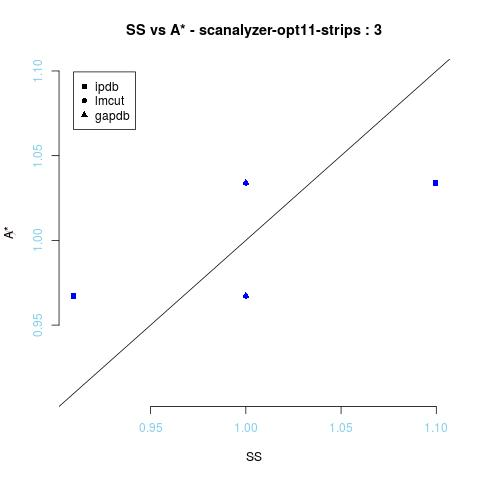
\includegraphics[width=\linewidth]{images/scanalyzer-opt11-strips}
\endminipage\hfill

%jump
\minipage{0.32\textwidth}
  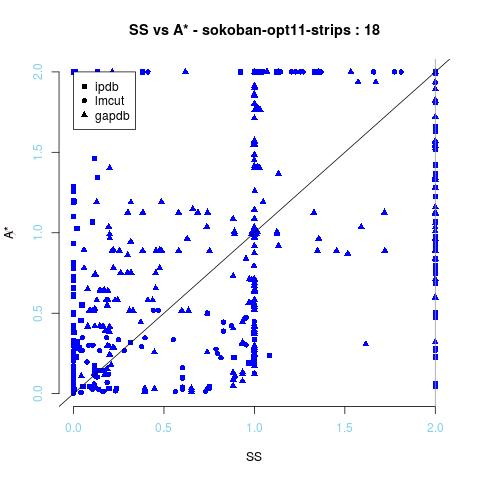
\includegraphics[width=\linewidth]{images/sokoban-opt11-strips}
\endminipage\hfill
\minipage{0.32\textwidth}
  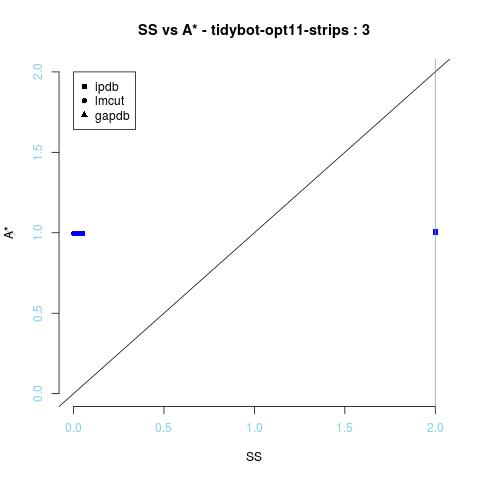
\includegraphics[width=\linewidth]{images/tidybot-opt11-strips}
\endminipage\hfill
\minipage{0.32\textwidth}
  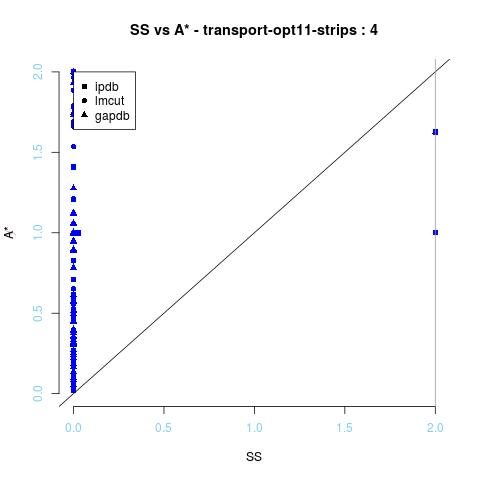
\includegraphics[width=\linewidth]{images/transport-opt11-strips} 
\endminipage\hfill

%jump
\minipage{0.32\textwidth}
  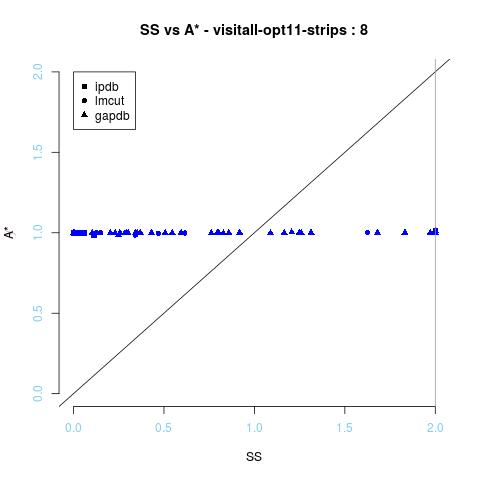
\includegraphics[width=\linewidth]{images/visitall-opt11-strips}
\endminipage\hfill
\minipage{0.32\textwidth}
  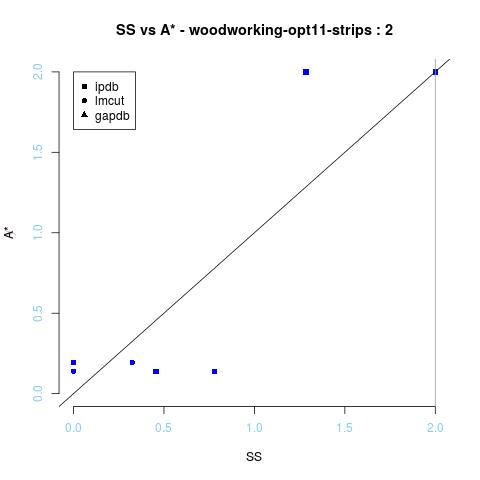
\includegraphics[width=\linewidth]{images/woodworking-opt11-strips}
\endminipage\hfill
\caption{\texttt{SS} vs A$\sp{*}$ ratios for the optimal domains $-$ The number of instances used in each domain are showed next to the name of the Domain.}\label{fig:img_analysis_domains}
\end{figure}

\newpage

In Table \ref{tb:per_ss_made_correctly} we present a single number for each domain representing the percentage of choices \texttt{SS} make correctly. From all the domains all are above of the 50$\%$ which means that at least the half of the points represent good relation of heuristics. With this experiment we prove that \texttt{SS} is not as bad as we thought it would be when we want to make selection.

\begin{table}[!htb]
\centering
\begin{tabular}{lc}
\hline
Domain      & II and III ($\%$) \\ \hline
Elevators   & 78.57    \\
Floortile   & 96.08    \\
Nomystery   & 71.82    \\
Parcprinter & 70.50    \\
Pegsol      & 96.83    \\
Scanalyzer  & 100.00   \\
Sokoban     & 89.31    \\
Tidybot     & 100.00   \\
Transport   & 51.78    \\
Visitall    & 98.05    \\
Woodworking & 100.00   \\ \hline
\end{tabular}
\caption{Percentage of choices \texttt{SS} made correctly.}
\label{tb:per_ss_made_correctly}
\end{table}

\clearpage